\documentclass[11pt]{amsart}
\usepackage{geometry}                % See geometry.pdf to learn the layout options. There are lots.
\geometry{letterpaper}                   % ... or a4paper or a5paper or ... 
%\geometry{landscape}                % Activate for for rotated page geometry
%\usepackage[parfill]{parskip}    % Activate to begin paragraphs with an empty line rather than an indent
\usepackage{graphicx}
\usepackage{amssymb}
\usepackage{epstopdf}
\usepackage{booktabs}
\DeclareGraphicsRule{.tif}{png}{.png}{`convert #1 `dirname #1`/`basename #1 .tif`.png}

\title{An Implementation of the Persistent Homology Transform for Metricizing Shapes}
\author{Hanyu Song and Azeem Zaman}
%\date{}                                           % Activate to display a given date or no date

\begin{document}
\maketitle
%\section{}
%\subsection{}
\section{Abstract}
Our goal was to develop a package to implement the results of the paper by Turner et. al. In particular, we wrote codes to compute the persistent homology transform (PHT) of an object in $\mathbb{R}^3$ and shapes in $\mathbb{R}^2$. PHT is a statistic that completely describes a shape or surface and allows us to determine a metric on the space of piecewise linear shapes, thereby possibly useful for statistical analysis such as clustering. 


\section{Background}
The paper introduces a tool that can be used to perform statistical shape analysis on objects in $\mathbb{R}^3$ and shapes in $\mathbb{R}^2$.  The result can be of interest to topological data analysists (TDA), researchers modeling shapes (such as medical imaging) and morphologists. One of the paper authors use this to compute the distance between heel bones in primates to generate a tree, which can be compared with a tree generated from the genetic distances between primate species.  

\section{Code Overview}
Here is a list of functions contained in the package:
\begin{enumerate}
\item{Functions to read in files containing the data}
\item{A function to construct a persistence diagram given a direction}
\item{Functions to calculate the distance between persistence diagrams}
\item{Functions to generate directions for the construction of persistence diagrams}
\item{Functions to caluclate the distance between objects}
\item{Functions to generate diagrams for many objects given a set of directions}
\item{Main function to be called by user}
\end{enumerate}
The following packages are required for implementation: \texttt{math, multiprocessing, numpy, scipy, glob} and \texttt{numba}.

\subsection{Functions for reading shapes}
Two functions for reading in data are included in the package. The first \texttt{read\_file} is for reading in text files saved with raw shape data; the second \texttt{read\_closed\_shape} is used to read Matlab \texttt{.mat} files saved with closed shape data. Note that each file contains the data of only one shape. Both functions can read all relevant files in a specified directory; both return a list of vertices and edges of each shape, with the vertices and edges saved in two separate \texttt{numpy.ndarray}'s.

\subsection{Functions for construction of persistence diagrams}
We wrote  to construct a persistence diagram given a direction is included in the package. Below are the detailed explanations of persistence diagrams.

A persistence diagram is a filtration.  We start with an object and "build" the object in a certain direction.  We record when each point in the object first appears (is "born") and when it merges into an object that already exists (it "dies).  Consider the shape below:
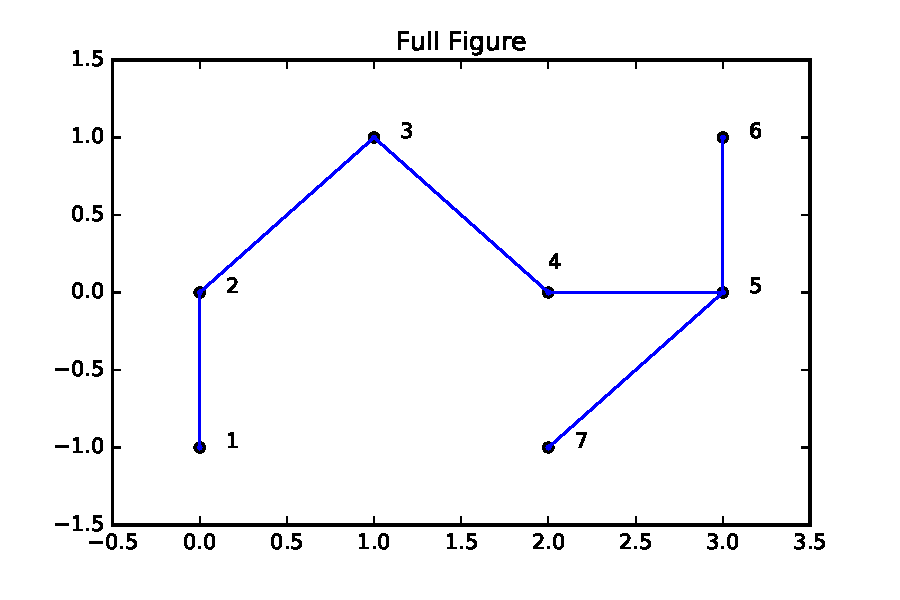
\includegraphics[width = \textwidth]{full_fig.pdf}

We will construct this figure in the direction $v = (0,1)$.  If we imagine moving upwards across the figure, the first height at which we will see any points of the diagram is $h=-1$.  We see that vertices 1 and 7 are born at $h = -1$, as shown below:

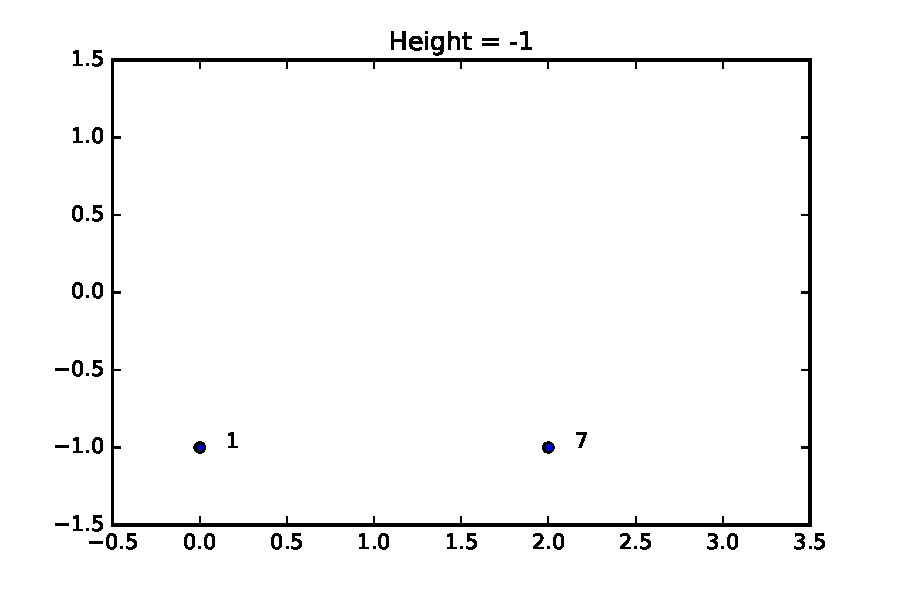
\includegraphics[width = \textwidth]{h1.pdf}

The next height at which something something interesting happens is $h = 0$, at which time three more points are born.  All of these points, however, die immediately.  Vertex 2 merges with vertex 1 and vertices 4 and 5 merge with vertex 7.  At this time we have two unconnected components.

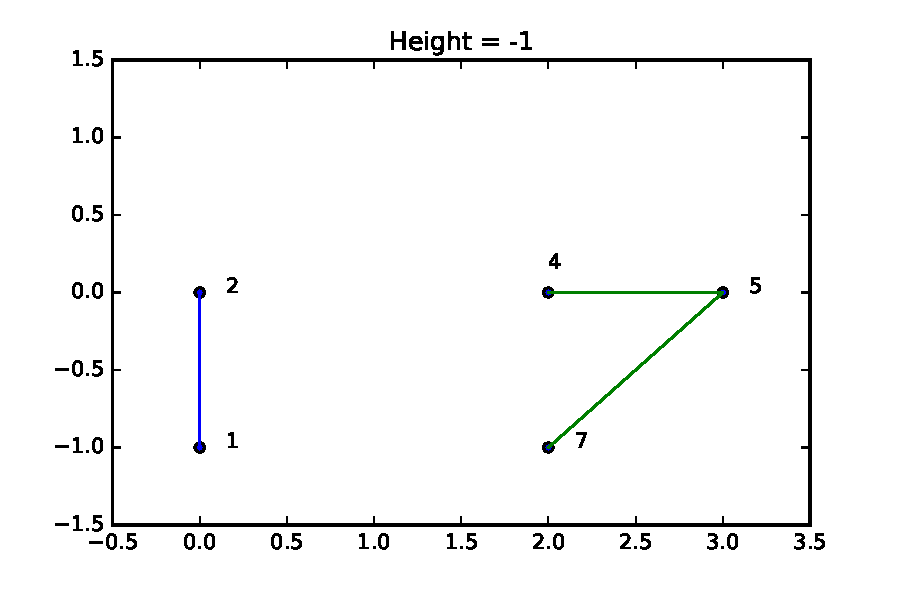
\includegraphics[width = \textwidth]{persist_diag2.pdf}

Once we reach $h = 1$, we have finished constructing the diagram.  Vertex 6 dies immediately because it merges with vertex 5.  Vertex 3 joints the two components that were previously disjoint.  Since vertices 1 and 7 were both born at $h=-1$, we make a convention that lower numbered vertices will be considered the root and higher numbered vertices will merge with them.  Thus at time $h=1$ vertex 7 dies, as it merges with vertex 1.

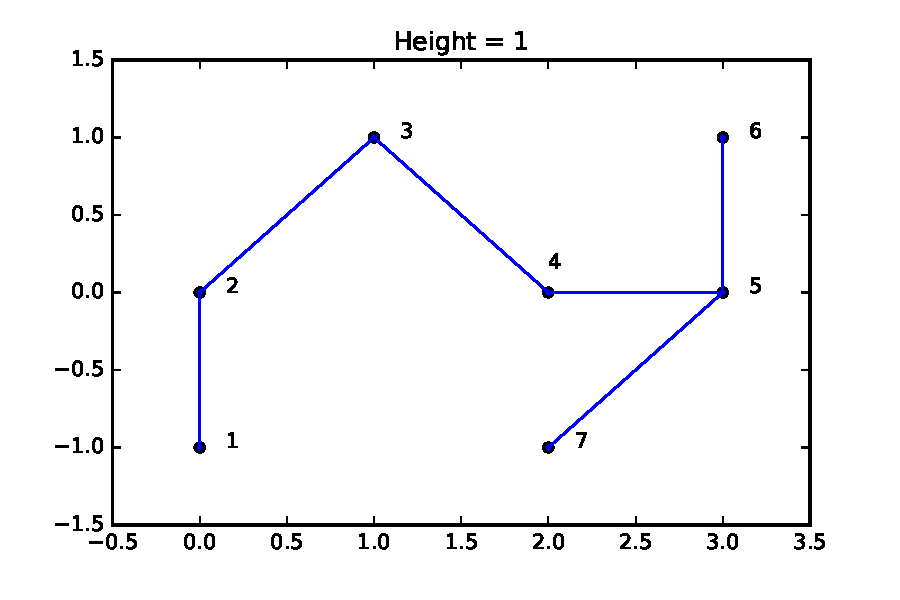
\includegraphics[width = \textwidth]{persist_diag3.pdf}

A plot of the persistence diagram is given below.  The red point represents vertex 1, which never dies.  We consider the point to be at $(-1,\infty)$.  The line in the figure is the diagonal.  A point on the diagonal is one that is born and dies at the same instant.  

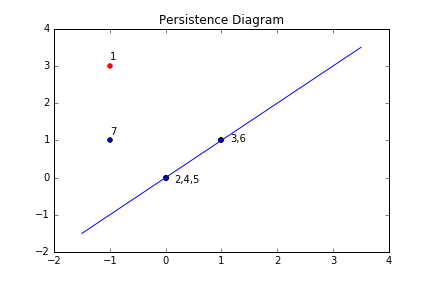
\includegraphics[width = \textwidth]{diagram.png}

To impliment this process of constructing persistence diagrams, we need to be able to tell when a vertex is born and when the vertex merges with another component.  For a fixed direction $v$ (which we will always take to be unit length), we can easily determien the height of a vertex. The height of a vertex $p$ with respect to a direction $v$ is simply the inner product of these two vectors.  

The harder part of the algorithm is determining when components merge.  To keep track of this, we will use a modified version of the Union-Find algorithm.  We define a class called \texttt{Tree}.  A \texttt{Tree} object has a parent and every tree begins with its own parent.  For convenience, it also has a name.  We will name a tree after a vertex.  So for each vertex $i$ there will be a tree such that \texttt{Tree.name = i}.  

The function \texttt{Find} finds the root of a tree by traveling up the tree until we find a tree that is equal to its parent.  The function \texttt{height\_Union} joins two trees in a specific way.  If the two input trees have the same root, nothing is done.  If the two trees have different heights, we make the root of one tree equal to the root of the other tree, effectively merging the trees.  As persistence diagrams are built upwards, we make the root of the joint tree the vertex that has the smaller height.  If the vertices have the same height, we make the root the vertex with the lower number.  

These functions are used internally and will not be called by a user.  

\begin{verbatim}
class Tree:
	def __init__(self, name):
		self.parent = self
		self.name = name
		self.rank = 0
	
def Find(x):
	"""
	This function determines the root of the tree
	that x is in.  It works recursively. x should
	be an object of class Tree.
	"""
	if x.parent != x:
		x.parent = Find(x.parent)	
	return x.parent

def height_Union(x, y, dict_heights):
	"""
	This function takes the union of two nodes.
	It does this by changing the root one tree
	to be the root of the other tree.  It changes the
	root based on height.  The root becomes the node with
	the lowest height.  So the node that is born first
	becomes the root.  

	If the two roots have the same height, the lowest 
	number becomes the root.  For example, if we have vertex
	1 and vertix 3 at the same height, vertex 1 will become
	the root.  

	Inputs:
		x,y:  objects of Tree class
		dict_heights:  a map v-> h, where v is a vertex,
		which should be the .name of some tree and h is
		the height with respect to some direction
        
    Returns:
        No returns.  Tree objects are merged.
	"""
	x_root = Find(x)
	y_root = Find(y)
	if x_root == y_root:
		return None
	if dict_heights[x_root.name] < dict_heights[y_root.name]:
		y_root.parent = x_root
	elif dict_heights[x_root.name] == dict_heights[y_root.name]:
		if x.name < y.name:
			y_root.parent = x_root
		else:
			x_root.parent = y_root
	else:
		x_root.parent = y_root
		
\end{verbatim}

\section{Distance between persistence diagrams}
Once we have a diagram, we can consider the distance between diagrams.  If $X$ and $Y$ are diagrams, we can consider bijections $\phi$ between the points and copies of the diagonal in $X$ with the points and copies of the diagonal in $Y$.  Bijections always exist because there are enought copies of the diagonal to create one.  We define the distance between $X$ and $Y$ to be
\begin{align}
dist_p(X,Y) &= \left(\inf_{\phi: X \to Y}\sum_{x \in X} ||x - \phi(x)||_p^p\right)^{1/p}.
\end{align}
The paper suggests that $p=1$ performs best in practice (the $L1$ norm).  The existence of an optimal bijection is proved in the literature.  An example of an optimal bijection is shown below (taken from www.math.uiuc.edu).  The points of $X$ are shown in red and the points of $Y$ are shown in blue.  The red points are paired with nearby blue points.  Most blue points are paired with their projection onto the diagonal.  In practice, we see that we add the projection onto the diagonal for each point.  This is an optimization problem that can be solved using the Hungarian (Munkres) algorithm.  We can calculate the distance between the points in $X$ and the points in $Y$ and the distance from the points in $X$ to the diagonal.  This can be represented as a cost matrix.  

As we will discuss in detail later, this is the bottleneck in our code.  The algorithm is somewhat difficult to implement, so we used an existing implementation.  Another difficulty is that the first implementation we tried got stuck in an infinite loop.  We settled on using a function from \texttt{scipy.optimize}, \texttt{linear\_sum\_assignment}.  This is the distance between the finite points.  We also need to consider the points with one component at infinity.  We will pair these amongst themselves and simply consider the distance between the birth times.  If two diagrams have a different number of points at infinity, then we would have to pair a point at infinity with a finite point or a point on the diagonal, which is infinitely far away.  The distance between such diagrams is said to be infinite.  

\section{Distance between objects}
Now that we can calculate the distance between two persistence diagrams, we are ready to compute the distance between two objects in $\mathbb{R}^2$ or $\mathbb{R}^3$.  For the objects we are considering, the distance (which is indeed a distance based on the results in the paper) is
\begin{align}
dist(M_1,M_2) := \int_{S^{d-1}} dist(X(M_1,v),X(M_2,v))\,dv,
\end{align}
where $X(M_i,v)$ is the persistence diagram for object $M_i$ in direction $v$.  Stability results from the paper reassure that the error in approximating the distance using only a finite sampling of directions should be small.  Thus we approximate this integral by using a sample of points from the circle (in $\mathbb{R}^2$) or the sphere (in $\mathbb{R}^3$).  

If is often useful to consider objects modulo a group of transformations, typically scaling, rotation, and translation.  Descriptions of how to implement these transformations can be found in the paper.  The code that centers and scales the objects is given below.  Rotation is slightly different.  To calculate the distance modulo rotation, we must consider all possible rotations of the second object and select the one that minimizes the distance.  In practice, we select some finite set of rotations to consider.  Furthermore, we do not actually rotate the object.  Instead, we note that the persistence diagram of a rotated object is the persistence diagram of a rotated direction.  Thus if we pick evenly spaced vectors, we simply need to relabel persistence diagrams to rotate objects.

\section{Algorithms}
One algorithm used is the Hungarian (or Munkres) algorithm.  The alogirthm is used in situations where assignments with an associated cost must be made and the goal is to select the assignment to minimize the cost.  Here we use this algorithm to calculate the distance between persistence diagrams. The distance between persistence diagrams is the sum of the distances between the points of the first persistence diagram paired with the points of the second diagram and additional points on the diagonal.  Selecting the pairing that minimzies this distance can be achieved using the Munkres algorithm.

Another algorithm used in our code is the Union-Find algorithm.  This algorithm is used in the construction of the persistence diagrams. During the construction we must keep track of when disjoint components merge.  We view each component as a tree.  When two components merge we join the roots of the trees.  This allows us to find when disjoint components merge.

\section{Tests and Examples}
\subsection{Test on simulated data}
In this section we test the functions on simple shapes, two squares and two triangles.  The shapes are similar, but they are slightly different in size and rotation.  We will use the scaling distance function to test whether we can cluster these shapes. The simpler shapes are shown below.
\begin{figure}
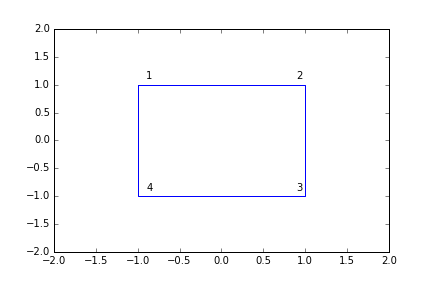
\includegraphics[width = .45\textwidth]{sqr1.png}
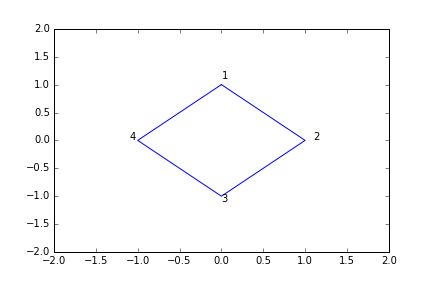
\includegraphics[width = .45\textwidth]{sqr2.png}
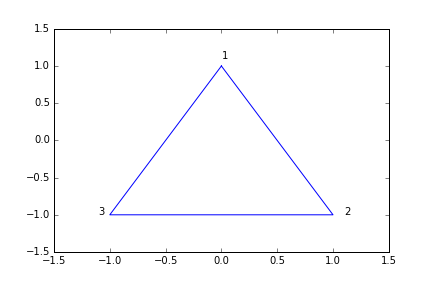
\includegraphics[width = .45\textwidth]{triag1.png}
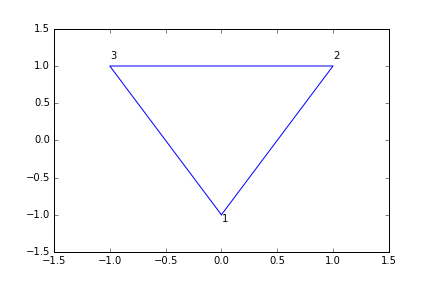
\includegraphics[width = .45\textwidth]{triag2.png}
\end{figure}

Our code generates the following distance matrix:
\begin{table}[]
\centering
\caption{Distance Matrix Generated by PHT}
\label{simptestdistl}
\begin{tabular}{@{}c|llll@{}}
\toprule
Shape                           & Square 1 & Square 2 & Triangle 1 & Triangle 2 \\ \midrule
Square 1                        & 0        & 0.00215  & 0.00530    & 0.00523    \\
Square 2                        & 0.00215  & 0        & 0.00530    & 0.00523    \\
Triangle 1                      & 0.00530  & 0.00530  & 0          & 0.00144    \\
\multicolumn{1}{l|}{Triangle 2} & 0.00523  & 0.00523  & 0.00144    & 0          \\ \bottomrule
\end{tabular}
\end{table}

We see that the distance between the triangles (the first two shapes) is less than the distance between the squares.  In fact, the distance between the triangle and the two squares is almost identical.  Similarly, the distance between the squares and both triangles are almost equal.  The distances here are so distinct that we can successively cluster the objects using simple hierarchical clustering.  


\section{Test on real data}
We will now test the code on real data from the MPEG-7 data set.  These are images that have been converted to outlines.  They are stored as \texttt{.mat} files, we will read them in using the function we wrote for that purpose.  The objects are displayed below.  We are testing the code on two objects from each of four different classes.  
\begin{figure}
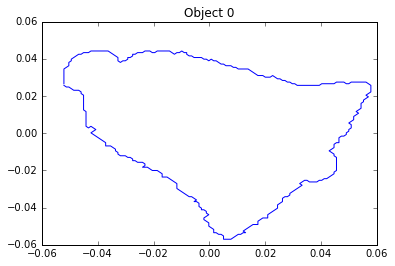
\includegraphics[width = .22\textwidth]{obj0.png}
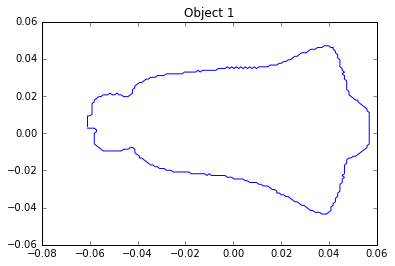
\includegraphics[width = .22\textwidth]{obj1.png}
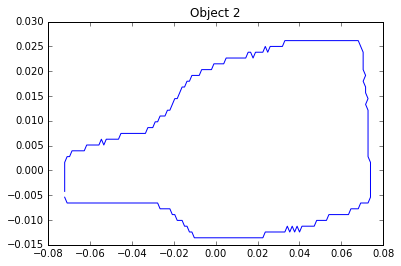
\includegraphics[width = .22\textwidth]{obj2.png}
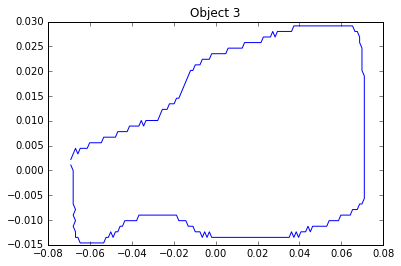
\includegraphics[width = .22\textwidth]{obj3.png}
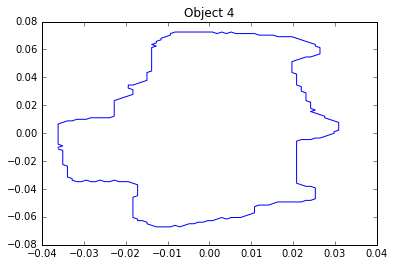
\includegraphics[width = .22\textwidth]{obj4.png}
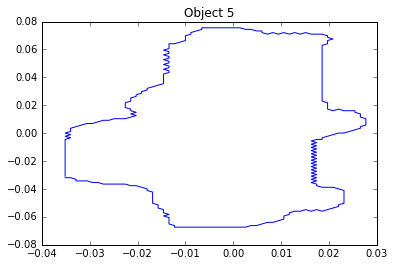
\includegraphics[width = .22\textwidth]{obj5.png}
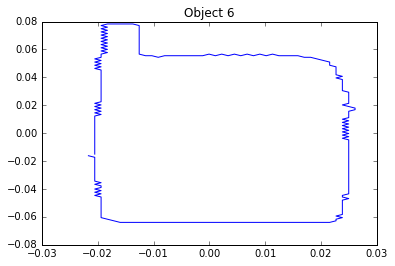
\includegraphics[width = .22\textwidth]{obj6.png}
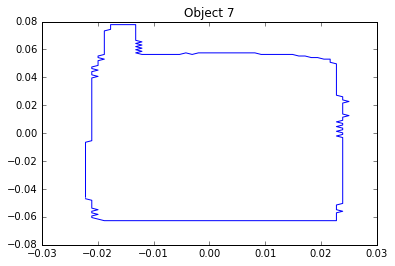
\includegraphics[width = .22\textwidth]{obj7.png}
\end{figure}
\begin{figure}
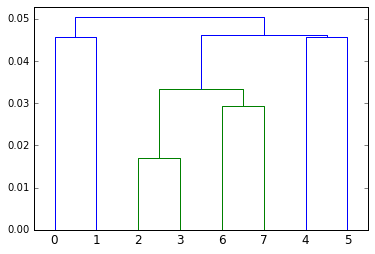
\includegraphics[width = \textwidth]{real_dendogram.png}
\end{figure}

\section{Optimization}
\subsection{Code Optimization}
We tried optimizing the performance of the codes using \texttt{numba} just-in-time (JIT) compilation, \texttt{Cython}, embarrassingly parallel processing. Based on the input file \texttt{Class1\_Sample1.mat}, most functions perform very well, taking only milliseconds to process such a shape with $375$ vertices. Assuming we want to measure the distance between such a shape to another shape with $375$ vertices, it takes $33.6s$ for the current Munkres algorithm to finish running, suggesting room for improvement.

We used the function \texttt{linear\_sum\_assignment} (Source: https://github.com/scipy/scipy/blob/master/scipy/optimize/\_hungarian.py\#L13-L107`scipy) from \texttt{scipy.optimize}. To improve its performance, we tried numba JIT computation, simple compilation in \texttt{Cython}, cythonizing via static typing and \texttt{cnumpy} iteration and wrapping \texttt{C} codes. However, no correct and easily accessible \texttt{C} or \texttt{C++} functions have been found. Neither have we achieve significant improvement in \texttt{Python}. Specifically, the major problem in cythonizing concerns the fast array declarations in \texttt{cdef} classes. Fast array declarations, however, are currently not accessible in the fields of cdef classes or as global variables, according to Cython documentation
(ref: http://cython.readthedocs.io/en/latest/src/tutorial/numpy.html).

We benchmarked the different optimization strategies based on a $1,000 \times 1,000$ cost matrix. The performances are  summarized in the table below:
\begin{table}[]
\centering
\caption{Function Speeds}
\label{my-label}
\begin{tabular}{@{}|c|l|l|l|l|@{}}
\toprule
Code      & Original Function & numba JIT & Cython    & Cython with static typing and \texttt{cNumPy} \\ \midrule
Wall Time & 1 min 41s         & 1 min 27s & 1 min 46s & 1 min 42s                                       \\ \bottomrule
\end{tabular}
\end{table}

\subsection{Algorithm Optimization}
We sped up the function \texttt{make\_diagram} via better algorithm. When constructing a \texttt{diagram}, we exclude points that are born and die at the same time,i.e. points that fall on the diagonal (as shown below), which largely reduces the size of the cost matrix, thereby leading to a significant speed-up of \texttt{linear\_sum\_assignment}, the function we discussed above.  THIS IS THE MOST IMPORTANT OPTIMIZATION IN THE CODE!

The chunk that helps speed up the function is shown below:
\begin{verbatim}
 for v in dict_heights.keys():
        # if time of death is none, add a point at infinity
        if dict_deaths[v] == None:
            diag.addinfpt(dict_heights[v])
        else:
            # only add point if not on the diagonal
            # this is designed to reduce the complexity
            # of the problem for the Munkres algorithm
            if dict_heights[v] != dict_deaths[v]:
                diag.addpt((dict_heights[v], dict_deaths[v]))
\end{verbatim}
\end{document}  